% chapter3.tex (Chapter 3 of the thesis)


\chapter{Compositions and Implementation of Techniques}
% In this chapter, I will present my folio and subsequent findings through the compositional process.
% This will be more broad, and I will make amendments to what I posited in Chapter 2. 
% \subsection{Background}
% Provide a better understanding on the ways that these techniques can be incorporated idiomatically into a composer's practice.

% \subsection{Research statement/problem}
% There is a dearth of resources for composers interested in these techniques, as evidenced by this research being novel.

% \subsection{Aim and scope of thesis}
% Ways to incorporate and present these techniques in an idiomatic way that is intuitive.

% \subsection{Significance of work}
% The properties of these techniques and the ways that they can be used idiomatically.

My folio of works comprises of four pieces. \nameref{sec:violaPiece}, for solo viola, \nameref{sec:bassPiece}, for solo contrabass, \nameref{sec:celloPiece}, for solo cello, and \nameref{sec:violinPiece}, for violin. 
These works all deal with different facets of the techniques that I have researched in this exegesis. 
Through the process of practice based research and reflection on the implementation of these pieces, it is hoped that a clear identity of idiomatic treatment of these techniques will be elucidated.
Shortcomings are still valuable data points due to the lack of information readily available about the treatment and usage of these techniques.
It is envisaged that these works are to be used as etudes, both for musicians as testing grounds for the capabilities of the techniques, and for composers seeking to study scores to better understand how to implement these techniques in their own works.
Through the process of journalling my compositional intent, it will become clear what the function of each piece is.
Comparisons and contrasts to pre-existing literature and works will support the techniques' idiomacy. 


\subsection{Background}
Implement the techniques in a musical context.
\subsection{Research statement/problem}
Compositions will show both how these techniques can be used idiomatically, and how they can inform my craft.
\subsection{Aim and scope of thesis}
Writing works which will increase the collective understanding of how to implement these techniques.
\subsection{Significance of work}
Incorporating these techniques into my compositional process will show the pitfalls and ways that these techniques can be used.

\section{\violinPiece} \label{sec:violinPiece}
\violinPiece is a solo work for violin that explores \hyperref[sec:halfHarmonicsDiscussion]{half-harmonics}.
It is a non-programmatic work, and the title was inspired by a question that my supervisor posed to me while I sought ethics approval for the exegesis.
Half-harmonics are perhaps one of the simplest techniques to achieve, produced by applying finger pressure halfway between that required to create a harmonic, and a \emph{normale} sound.
This means that the scale of finger pressure is thus;

\begin{table}[]
    \centering
    \caption{Finger Pressure \& Resultant Sound}
    \label{tab:finger-pressure}
    % \resizebox{\textwidth}{!}{%
    \begin{tabular}{@{}ll@{}}
    \toprule
    Finger pressure & Result        \\ \midrule
    Open            & Fundamental   \\
    Touching        & Harmonic      \\
    More pressure   & Half-harmonic \\
    Fingerboard     & Normale       \\ \bottomrule
    \end{tabular}%
    % }
    \end{table}

The one-dimensional nature of this facet of the techniques leaves little variability in the implementation of the technique. 
Thus, \violinPiece explores the relationship between half-harmonics and other finger pressures. 
Rapid change between half-harmonics, regular harmonics, and \emph{normale} makes the work an exercise in finger control, as well as an introductory work to half-harmonics.
Below, I demonstrate the rapid changes of the half-harmonics in mm. 5 of \violinPiece.

% TODO: Add in picture of half harmonics  - https://trello.com/c/cYTkFAaV/27-add-in-picture-of-half-harmonics
\begin{figure}
    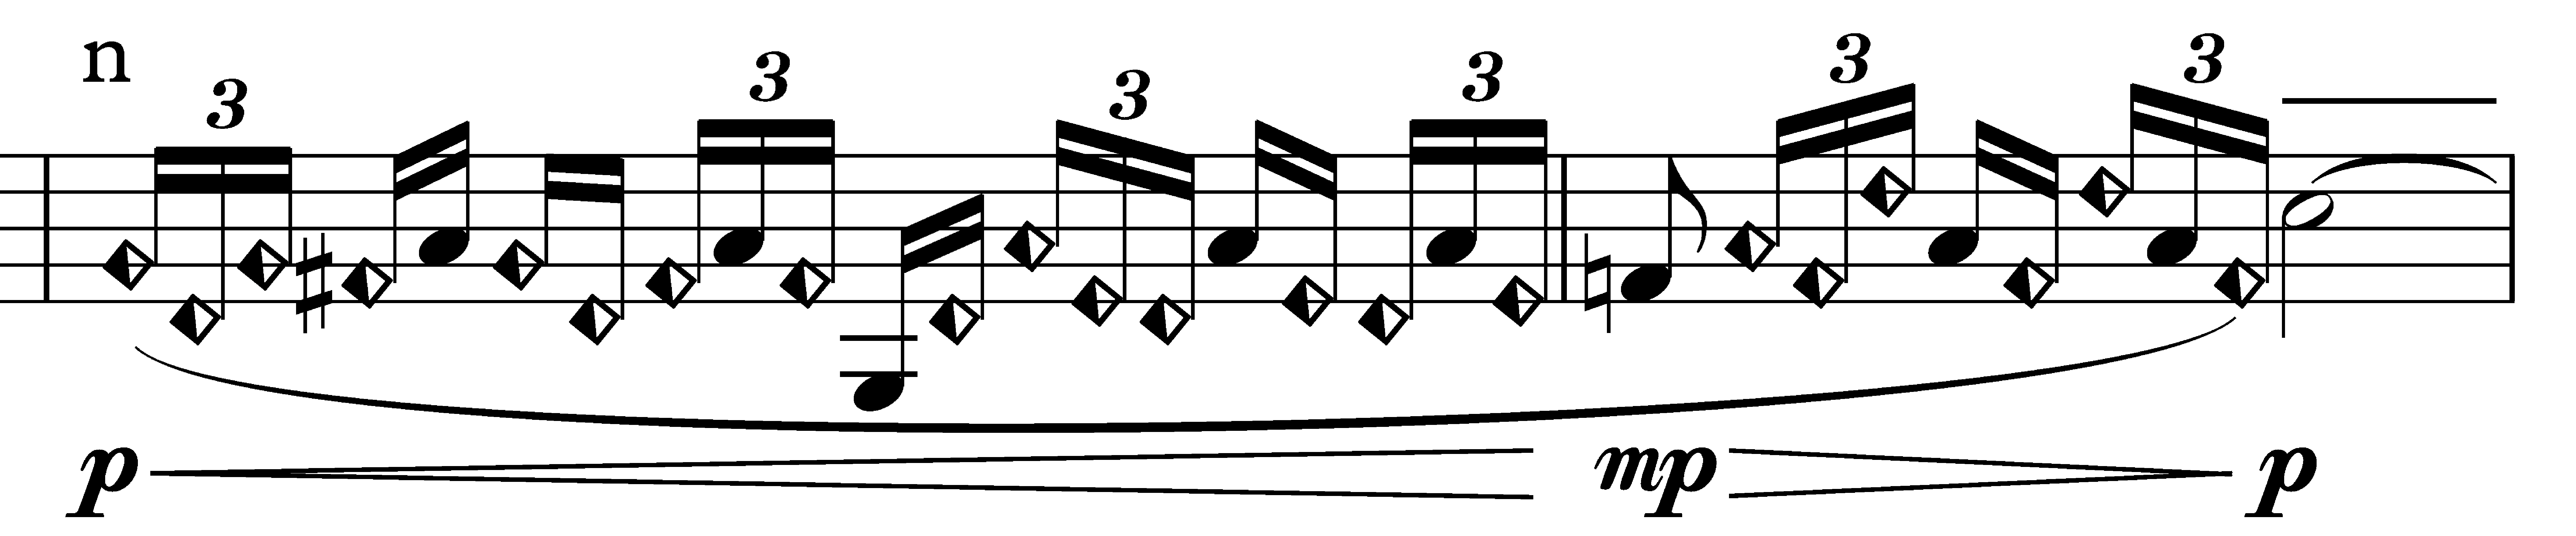
\includegraphics[width=\linewidth]{./resources/violinHalfHarmonicsExcerpt5.pdf}
    \caption{Excerpt from \violinPiece}
  \label{fig:Excerpt from what are you doing with the humans, mm. 5}
  \end{figure}

\violinPiece takes inspiration from Sciarrino's fifth Caprice, and serves as a stepping stone to the more difficult Caprice.\autocite[]{sciarrinoCapricciViolino1976} 
In practice, the pitch content of my work was obscured by the glassy texture of half-harmonics, rendering large portions of it as noise. 
With the knowledge that properly performed, the harmonic content would be obscured, I leant into this, writing in a more tonal style than I do usually.
Another facet of half-harmonics that I wanted to explore was the timbral aspect of them, bar 27 shown in Figure ~\ref{fig:violinHalfHarmonicsExcerpt27}.
Similar to a multiphonic in their rich harmonic content, half-harmonics do not have the purity of tone that regular harmonics have.
I explore the interplay of half-harmonics, regular harmonics, and \emph{normale}, double stopped minims and semibreves slowly changing from one mode of pressure to another.
In this way, violinists that play \violinPiece will become familiar with different modes of pressure played concurrently.

\begin{figure}
    
\includegraphics[width=\linewidth]{./resources/violinHalfHarmonicsExcerpt27.pdf}
    \caption{Excerpt from \violinPiece} \label{fig:violinHalfHarmonicsExcerpt27}
  \end{figure}

Notationally, the rapid changes between half-harmonics and other techniques were an ideal testing ground for different notation types. 
Notably, the issue of half-filled diamond noteheads not having any distinction between crotchets and minims is not an issue due to the rapidity of the work.
Below is a passage, with three different methods of notating the half-harmonics.


Ultimately, I opted to implement the half-filled diamond noteheads, finding them to most accurately present the information in a way that was inobtrusive, and built upon pre-existing notation.
It should be noted that this is contrary to the opinion set out in Dimpker's seminal thesis on notation, \emph{Extended notation. The depiction of the
unconventional}, but conforms to Gould's opinion on the matter.\autocites[120-121]{dimpkerExtendedNotationDepiction2012}[61]{gouldBars2011}
% TODO: fix gould citation - https://trello.com/c/gYLN8lqN/28-fix-gould-citation

\section{\violaPiece} \label{sec:violaPiece}
% TODO: Write Doppelganger
\violaPiece is a piece for solo viola, written to explore the lower register of the viola using \hyperref[sec:subharmonicsDiscussion]{subharmonics} juxtaposed with upper harmonics. 
I wanted to explore the extreme ranges of the viola,


\subsection{Findings of \emph{Doppelganger}}
Workshopping an early draft of \emph{Doppelganger} with a violist, I found that the pressure needed to `find' a subharmonic was fleeting, and could not be reproduced for long periods of time.
As such, I amended the score to treat subharmonics largely as a `special effect', and not ascribe importance to their pitched content.


\section{\celloPiece} \label{sec:celloPiece}

\celloPiece is \lipsum[1]


\section{\bassPiece} \label{sec:bassPiece}
% TODO: Write The Veldt
Inspired by the eponymous short story by Ray Bradbury, \bassPiece  is a composition for solo contrabass with electronics. 
Similarly like the namesake, this world is filled with danger but also beauty. 
It is non-programmatic, and my intent with Veldt was to create a soundworld and space that the performer was able to `roam around' in, and features several sections of improvisation on pitch-sets.

\subsection{Findings of \emph{The Veldt}}
Writing for contrabass, I found subharmonics came most easily on the G string. 
